% \documentclass[12pt, twoside]{article}
\usepackage[letterpaper, margin=1in, headsep=0.2in]{geometry}
\setlength{\headheight}{0.6in}
%\usepackage[english]{babel}
\usepackage[utf8]{inputenc}
\usepackage{microtype}
\usepackage{amsmath}
\usepackage{amssymb}
%\usepackage{amsfonts}
\usepackage[nomessages]{fp} %\FPeval{\var-name}{2*sin(pi/6)}
\usepackage{siunitx} %units in math. eg 20\milli\meter
\usepackage{yhmath} % for arcs, overparenth command
\usepackage{tikz} %graphics
\usetikzlibrary{quotes, angles, arrows, arrows.meta}
\usepackage{graphicx} %consider setting \graphicspath{{images/}}
\usepackage{parskip} %no paragraph indent
\usepackage{enumitem}
\usepackage{multicol}
\usepackage{venndiagram}

\usepackage{fancyhdr}
\pagestyle{fancy}
\fancyhf{}
\renewcommand{\headrulewidth}{0pt} % disable the underline of the header
\raggedbottom
\hfuzz=2mm %suppresses overfull box warnings

\usepackage{hyperref}

\fancyhead[LE]{\thepage}
\fancyhead[RO]{\thepage \\ Name: \hspace{4cm} \,\\}
\fancyhead[LO]{BECA / Dr. Huson / Geometry\\*  Unit 11: Circle angles, sectors, arcs \\* 7 March 2023}

\begin{document}

\subsubsection*{11.7 Homework: Circle Angles}
\begin{enumerate}
\item Given $A(-1,2)$ and $B(-6,14)$, find the length of $\overline{AB}$. Show the substitution into the distance formula.
  %https://graspablemath.com/canvas?load=_024bda2a5587c074

\item Two lines intersect to make four angles: $\angle 1$, $\angle 2$, $\angle 3$, and $\angle 4$, as shown.
  \begin{multicols}{2}  
    \begin{enumerate}
      \item How are $\angle 1$ and $\angle 2$ related?
        \begin{itemize}
          %\renewcommand{\labelitemi}{$\square$}
          \item[$\square$] Vertical angles
          \item[$\square$] Complementary angles
          \item[$\square$] Supplementary angles
          \item[$\square$] Opposite angles
          \item[$\square$] Linear pair
        \end{itemize}
      \item Given $m\angle 1 = 75^\circ$.
        \begin{enumerate}
          \item Find $m\angle 3$ \vspace{0.5cm}
          \item Find $m\angle 4$ \vspace{2cm}
        \end{enumerate} 
        \end{enumerate}
    \begin{tikzpicture}[scale=0.7, rotate=30]
    \draw [<->, thick] (0,-1.5)--(10,1.5);
    \draw [<->, thick] (2,3.5)--(7,-3.5);
    \node at (3,.4){1};
    \node at (6,-.6){3};
    \node at (5,1){2};
    \node at (4,-1){4};
  \end{tikzpicture}
  \end{multicols}
  
\item A regular heptagon (7 sides) is inscribed in a circle with a radius $r=14$. Find each value (in terms of $\pi$ unless otherwise instructed).
  \begin{multicols}{2}
  \raggedcolumns
  \begin{enumerate}[itemsep=1.1cm]
    \item $m \angle AOB$ to the \emph{nearest degree}.
    \item The circle circumference. ($C=2\pi r$)
    \item The length of the arc $\wideparen{AB}$
    \item The circle's area. ($A=\pi r^2$)
    \item The sector area (shaded)
  \end{enumerate}
  \begin{tikzpicture}[scale=0.8]
    \fill [lightgray]
    (0,0)--(0:4) arc (0:51:4)--(0,0);
    \draw (0,0) circle[radius=4];
    \draw [thick, <->] (0:0.75) arc (0:51:0.75);
    \draw [thick, dotted]
    (0:4) node[right] {$A$}--
    (0,0) node[left] {$O$}--
    (51:4) node[above right] {$B$};
    \draw [thick]
    (0:4) -- (51:4)-- (103:4)-- (154:4)-- (206:4)-- (257:4)-- (309:4)-- cycle;
    \fill (0,0) circle[radius=.1];
    \node at (25:1.2) {$?$};
    \node at (-10:1.8) {$14$};
  \end{tikzpicture}
  \end{multicols}

\item Given circle $P$ with $m \wideparen{AB}=54^\circ$.
  \begin{multicols}{2}
    \raggedcolumns
    \begin{enumerate}
      \item Write down the $m\angle APB$. \vspace{1.7cm}
      \item Find the $m\angle AQB$. \vspace{2cm}
    \end{enumerate}
      \begin{tikzpicture}[scale=.6, rotate=60]
        \draw [thick] (0,0) circle[radius=5];
        \fill (0,0) circle[radius=.1];
        \draw [thick]
        (56:5) node[above] {$B$}--
        (0,0) node[below left] {$P$}--
        (110:5) node[above left] {$A$};
        \draw [thick] (56:5)--(190:5) node[below] {$Q$}--(110:5);
        \fill (190:5) circle[radius=.1];
        \draw (85:6.2) node[right]{$54^\circ$};
      \end{tikzpicture}
  \end{multicols}

\item A circle on the coordinate plane has center $C$ and radius $\overline {CT}$. A tangent line through point $T$ is drawn, as shown.
\begin{multicols}{2}
  \begin{enumerate}[itemsep=1.25cm]
    \item Write down the center of the circle as a coordinate pair.
    \item Write down the equation of the circle.
    \item What is the slope of the radius $\overline {CT}$?
    \item Find the slope of the tangent line.
  \end{enumerate}
    \vspace{2cm}
    \begin{flushright}
    \begin{tikzpicture}[scale=0.7]
      \draw [help lines] (-0.15,-2) grid (11,8);
      \draw [thick, ->] (-0.2,0) -- (11.4,0) node [above] {$x$};
      \foreach \x in {1,2,3,4,5,6,7,8,9,10,11}
        \draw[shift={(\x,0)},color=black] (0pt,2pt) -- (0pt,-2pt) node[below] {\footnotesize \; $\x$};
      \draw [thick, ->] (0,-2.2)--(0,8.4) node [left] {$y$};
      \foreach \y in {-1,1,2,3,4,5,6,7,8}
        \draw[shift={(0,\y)},color=black] (-2pt,0pt) -- (2pt,0pt) node[left] {\footnotesize \; $\y$};
      \draw [thick] (6,3) circle [radius=5];
      \draw [fill] (6,3) circle [radius=0.1] node[above right] {$C$};
      \draw [fill] (3,7) circle [radius=0.1] node[above left] {$T$};
      \draw [-, thick] (6,3)--(3,7);
      \draw [<->, thick] (-0.6,4.3)--(5,8.5);
    \end{tikzpicture}
    \end{flushright}
\end{multicols}

\item Two supplementary angles have measures $m\angle ABD = 3x$ and $m\angle DBC = 4x + 61^\circ$. \\[0.25cm] 
Write an equation applying the angle addition theorem, then find $x$. \vspace{0.5cm}
  \begin{flushright}
    \begin{tikzpicture}[scale=1]
      \draw [<->, thick]
        (0:3) coordinate (a) node[below left] {$C$}
        -- (0,0) coordinate (b) node[below] {$B$}
        -- (125:3) coordinate (c) node[above right] {$D$}
        pic["$4x+61^\circ$", <->, draw=black, angle eccentricity=1.5, angle radius=1cm]
        {angle=a--b--c};
        \draw [<-, thick]
        (180:4) coordinate (d) node[below] {$A$}
        -- (0,0) coordinate (e)
        pic["$3x$", <->, draw=black, angle eccentricity=1.5, angle radius=1cm]
        {angle=c--e--d};
    \end{tikzpicture}
  \end{flushright}
  %https://graspablemath.com/canvas?load=_324d9aa72a142273

\item Given circle with center $I$ and $m \wideparen{KT}=64^\circ$. Find the measure of each angle.
  \begin{multicols}{2}
    \raggedcolumns
    \begin{enumerate}[itemsep=1cm]
      \item $m\angle KIT$
      \item $m\angle KAT$
      \item $m\angle TIA$
      \item $m\angle ATI$
    \end{enumerate}
      \begin{tikzpicture}[scale=.65, rotate=30]
        \draw (0,0) circle[radius=5];
        \fill (0,0) circle[radius=.1];
        \draw [thick]
        (190:5) node[below left] {$K$}--
        (0,0) node[below] {$I$}--
        (130:5) node[above left] {$T$};
        \draw [thick] (0,0)--(10:5) node[above right] {$A$}--(130:5);
        \draw (155:5) node[left]{$64^\circ$};
        \draw [thick, <->] (130:1) arc (130:190:1);
        \draw [thick, <->] (10:3.5) arc (190:145:1);
      \end{tikzpicture}
  \end{multicols}

\item The shaded sector of the unit circle is \emph{one fifth} of the whole circle, as shown. \\(Circle circumference and area formulas: $C=2\pi r$, $A=\pi r^2$)
  \begin{multicols}{2}
  \raggedcolumns
  \begin{enumerate}[itemsep=1.5cm]
    \item Find $m \angle AOB$ in \emph{degrees}.
    \item Find the length of the arc $\wideparen{AB}$ in terms of $\pi$.
    \item Find the area of the shaded sector in terms of $\pi$.
  \end{enumerate}
  \begin{tikzpicture}[scale=0.8]
    \fill [lightgray]
    (0,0)--(0:4) arc (0:72:4)--(0,0);
    \draw (0,0) circle[radius=4];
    \draw [thick, <->] (0:1) arc (0:72:1);
    \draw [thick] (0:4) arc (0:72:4);
    \draw [thick]
    (0:4) node[right] {$A$}--
    (0,0) node[left] {$O$}--
    (72:4) node[above] {$B$};
    \draw [thick, dotted](72:4)--(0,0);--(108:4);
    \draw [thick, dotted](144:4)--(0,0);--(180:4);
    \draw [thick, dotted](-72:4)--(0,0);--(-108:4);
    \draw [thick, dotted](-144:4)--(0,0);
    \fill (0,0) circle[radius=.1];
    %\node at (18:4.5) {$?$};
    \node at (-10:2) {$1$};
  \end{tikzpicture}
  \end{multicols}

\item Given a triangle $\triangle ABC$ having angles with measures $m\angle A = 42^\circ$ and $m\angle B = 89^\circ$. Find the measure of the third angle, $m\angle C$.
  
\item The \emph{pie chart} below shows the proportion of two subsets of a population, one represented in blue and one in orange. Dotted lines divide the circle in ten equal sectors for reference.
  \begin{multicols}{2}
  \raggedcolumns
  \begin{enumerate}[itemsep=1.5cm]
    \item Estimate the area of the blue sector as a fraction of the circle and as a decimal.
    \item The central angle of the orange sector measures $50^\circ$. Find the fraction of circle's area shaded orange as a fraction and a decimal.
  \end{enumerate}
  \begin{tikzpicture}[scale=0.8]
    \filldraw [color=blue, fill=blue!20, thick]
    (0,0)--(36:4) arc (36:144:4)--(0,0);
    \draw (0,0) circle[radius=4];
    %\draw [thick] (0:4) arc (0:36:4);
    %\draw [thick]
    %(0:4) node[right] {$A$}--
    %(0,0) node[below left] {$O$}--
    %(36:4) node[right] {$B$};
    \draw [thick, dotted](72:4)--(0,0)--(108:4);
    \draw [thick, dotted](144:4)--(0,0)--(180:4);
    \draw [thick, dotted](-72:4)--(0,0)--(-108:4);
    \draw [thick, dotted](0:4)--(0,0)--(-144:4);
    \filldraw [color=orange, fill=orange!20, thick]
    (0,0)--(-10:4) arc (-10:-60:4)--(0,0);
    \draw [thick, <->] (-10:1) arc (-10:-60:1);
    \node at (-35:1.5) {$50^\circ$};
  \end{tikzpicture}
  \end{multicols}

\item Given circle with center $O$ and $m\angle QPR=39^\circ$. Find the measure of each arc or angle.
  \begin{multicols}{2}
    \raggedcolumns
    \begin{enumerate}[itemsep=1cm]
      \item $m \wideparen{QR}$
      \item $m\angle PQO$
      \item $m\angle QOR$
      \item $m\angle POQ$
    \end{enumerate}
      \begin{tikzpicture}[scale=.65, rotate=120]
        \draw (0,0) circle[radius=5];
        \fill (0,0) circle[radius=.1];
        \draw [thick]
        (190:5) node[below right] {$R$}--
        (0,0) node[above right] {$O$}--
        (110:5) node[below left] {$Q$};
        \draw [thick] (0,0)--(10:5) node[above left] {$P$}--(110:5);
        \draw (15:2.5) node[left]{$39^\circ$};
        \draw [thick, <->] (110:5) arc (110:190:5);
        \draw [thick, <->] (10:3.5) arc (190:130:1);
      \end{tikzpicture}
  \end{multicols}

\item The \emph{pie chart} below represents the population of the city of New York, with each borough's population a proportional sector.
  \begin{multicols}{2}
  \raggedcolumns
  Population of NY City is 8,336,000\\
  Population of Brooklyn is 2,560,000
  \begin{enumerate}%[itemsep=1.5cm]
    \item Find the fraction of New Yorkers, $x$, who reside in Brooklyn as a percentage. \vspace{2cm}
    \item Find the central angle of the shaded area, $\theta = x \times 360^\circ$
  \end{enumerate}
  \columnbreak
  \begin{flushright}
    New York City
  \begin{tikzpicture}[scale=0.8]
    \fill [lightgray]
    (0,0)--(0:4) arc (0:110:4)--(0,0);
    \draw (0,0) circle[radius=4];
    \draw [thick, <->] (0:1) arc (0:110:1);
    \draw [thick] (0:4) arc (0:110:4);
    \draw [thick]
    (0:4)--(0,0)--(110:4);
    %\draw [thick, dotted](72:4)--(0,0)--(108:4);
    %\draw [thick, dotted](144:4)--(0,0)--(180:4);
    \draw [thick, dotted](208:4)--(0,0)--(278:4);
    \draw [thick, dotted](-20:4)--(0,0)--(-82:4);
    \fill (0,0) circle[radius=.1];
    \node at (40:1.4) {$\theta^\circ$};
    \node at (60:2.5) {Brooklyn};
    \node at (170:2.5) {Queens};
    \node at (240:2.5) {Manhattan};
    \node at (-50:2.5) {Bronx};
    \node at (-7:3.2) {Staten Island};
  \end{tikzpicture}
  \end{flushright}
  \end{multicols}

\item Right $\triangle ABC$ is drawn in \emph{standard position} with vertex $A$ on the origin and right $\angle C$ on the $x$-axis, as shown.
\begin{multicols}{2}
  \raggedcolumns
\begin{enumerate}
  \item Find the length of the hypotenuse $AB$ using the Pythagorean Theorem $a^2 + b^2 = c^2$. (leave as a radical)
  \vspace{3cm}
  \item Find the slope of the line segment $\overline{AB}$ as a decimal.
\end{enumerate}
  \begin{tikzpicture}[scale=0.7]
    %\draw [help lines] (-1.15,-1.2) grid (11,10);
    \draw [thick, ->] (-0.2,0) -- (9.4,0) node [above] {$x$};
    \foreach \x in {1,2,...,9}
      \draw[shift={(\x,0)},color=black] (0pt,2pt) -- (0pt,-2pt) node[below] {\footnotesize \; $\x$};
    \draw [thick, ->] (0,-0.2)--(0,9.6) node [left] {$y$};
    \foreach \y in {1,2,...,9}
      \draw[shift={(0,\y)},color=black] (-2pt,0pt) -- (2pt,0pt) node[left] {\footnotesize \; $\y$};
    \draw [-, thick] (0,0) node[below left] {$A$}
    --(6,0) node[above right] {$C$}
    --(6,9)node[right] {$B (6,9)$}--cycle;
    \draw (6,0)++ (-0.5,0)-- +(0,0.5)-- +(0.5,0.5);
    %\draw [<->, thick] (-0.6,4.3)--(5,8.5);
  \end{tikzpicture}
\end{multicols}
%https://graspablemath.com/canvas?load=_024bda2a5587c074

\newpage
\item Convert between units. \\[0.25cm]
General method: if $A = B$ multiply by $\displaystyle \frac{A}{B} \text{ or } \frac{B}{A}$. For example, $\pi \text{ radians}= 180 \text{ degrees}$ so \\
$\displaystyle r = d \times \frac{\pi}{180}$ and 
$\displaystyle d = r \times \frac{180}{\pi}$
\vspace{0.5cm}
  \begin{multicols}{2}
  \raggedcolumns
  \begin{enumerate}[itemsep=1.5cm]
    \item $35^\circ = \hspace{0.15cm} ?$ radians
    \item $\displaystyle \frac{\pi}{9}  = \hspace{0.15cm} ?$ degrees
    \item 1 foot = 12 inches\\[0.5cm]
    4.25 feet = 
    \item 70 inches = 
    \item 1 euro = 1.21 dollars\\[0.5cm]
    50 euro = 
    \item 50 dollars = 
    \item 1 mile = 5,280 feet\\[0.5cm]
    11,000 feet = 
    \item $\displaystyle \frac{3}{4}$ mile =   
  \end{enumerate}
  \end{multicols}
 
\item Line segment $\overline{AB}$, $A(2,1)$, $B(10,7)$, is the diameter of circle $M$. 
\begin{enumerate}
  \item On the grid, mark and label as a coordinate pair the midpoint of the segment, the circle center $M$. 
  \item Calculate the length of $\overline{AB}$ and hence, the radius of the circle.\
  \item Write down the equation of the circle. 
  \item Sketch the circle on the grid or draw it with Geogebra or Graspable Math.
  \end{enumerate}
  \begin{flushright}
    \begin{tikzpicture}[scale=0.7]
      \draw [help lines] (-1.15,-1.2) grid (11,10);
      \draw [thick, ->] (-1.2,0) -- (11.4,0) node [above] {$x$};
      \foreach \x in {-1,0,...,10}
        \draw[shift={(\x,0)},color=black] (0pt,2pt) -- (0pt,-2pt) node[below] {\footnotesize \; $\x$};
      \draw [thick, ->] (0,-1.2)--(0,10.4) node [left] {$y$};
      \foreach \y in {-1,0,1,...,9, 10}
        \draw[shift={(0,\y)},color=black] (-2pt,0pt) -- (2pt,0pt) node[left] {\footnotesize \; $\y$};
      %\draw [thick] (6,3) circle [radius=5];
      \draw [fill] (2,1) circle [radius=0.1] node[below left] {$A$};
      \draw [fill] (10,7) circle [radius=0.1] node[above right] {$B$};
      \draw [-, thick] (2,1)--(10,7);
      %\draw [<->, thick] (-0.6,4.3)--(5,8.5);
    \end{tikzpicture}
    \end{flushright}
    %https://graspablemath.com/canvas?load=_024bda2a5587c074
    %https://graspablemath.com/canvas?load=_6a89b545540e2be5

  \item The shaded sector of the unit circle is \emph{one eighth} of the whole circle, as shown. \\(Circle circumference and area formulas: $C=2\pi r$, $A=\pi r^2$)
  \begin{multicols}{2}
  \raggedcolumns
  \begin{enumerate}[itemsep=1.5cm]
    \item Find $m \angle AOB$ in \emph{degrees}.
    \item Find the length of the arc $\wideparen{AB}$ in terms of $\pi$.
    \item Find the area of the shaded sector in terms of $\pi$.
  \end{enumerate}
  \begin{tikzpicture}[scale=0.8]
    \fill [lightgray]
    (0,0)--(0:4) arc (0:45:4)--(0,0);
    \draw (0,0) circle[radius=4];
    \draw [thick, <->] (0:1) arc (0:45:1);
    \draw [thick] (0:4) arc (0:45:4);
    \draw [thick]
    (0:4) node[right] {$A$}--
    (0,0) node[left] {$O$}--
    (45:4) node[above right] {$B$};
    \draw [thick, dotted](90:4)--(0,0)--(135:4);
    \draw [thick, dotted](225:4)--(0,0)--(180:4);
    \draw [thick, dotted](-45:4)--(0,0)--(-90:4);
    %\draw [thick, dotted](-135:4)--(0,0);
    \fill (0,0) circle[radius=.1];
    %\node at (18:4.5) {$?$};
    \node at (-10:2) {$1$};
  \end{tikzpicture}
  \end{multicols}

\item Given a triangle $\triangle ABC$ having angles with measures $m\angle A = 37^\circ$ and $m\angle B = 78^\circ$. Find the measure of the third angle, $m\angle C$.
  
\item The \emph{pie chart} below shows the proportion of two subsets of a population, one represented in blue and one in orange. Dotted lines divide the circle in six equal sectors for reference.
  \begin{multicols}{2}
  \raggedcolumns
  \begin{enumerate}[itemsep=1.5cm]
    \item Estimate the area of the blue sector as a fraction of the circle and as a decimal.
    \item The central angle of the orange sector measures $70^\circ$. Find the fraction of circle's area shaded orange as a fraction and a decimal.
  \end{enumerate}
  \begin{tikzpicture}[scale=0.8]
    \filldraw [color=blue, fill=blue!20, thick]
    (0,0)--(0:4) arc (0:120:4)--(0,0);
    \draw (0,0) circle[radius=4];
    \filldraw [color=orange, fill=orange!20, thick]
    (0,0)--(-10:4) arc (-10:-80:4)--(0,0);
    \draw [thick, <->] (-10:1) arc (-10:-80:1);
    \node at (-40:1.5) {$70^\circ$};
    \draw [thick, dotted](60:4)--(0,0)--(180:4);
    %\draw [thick, dotted](144:4)--(0,0)--(180:4);
    \draw [thick, dotted](-60:4)--(0,0)--(-120:4);
    %\draw [thick, dotted](0:4)--(0,0)--(-144:4);
  \end{tikzpicture}
  \end{multicols}

\item Given circle with center $O$ and $m\angle QPR=31^\circ$. Find the measure of each arc or angle.
  \begin{multicols}{2}
    \raggedcolumns
    \begin{enumerate}[itemsep=1cm]
      \item $m \wideparen{QR}$
      \item $m\angle QOR$
      \item $m\angle POQ$
      \item $m\angle PQO$
    \end{enumerate}
      \begin{tikzpicture}[scale=.65, rotate=160]
        \draw (0,0) circle[radius=5];
        \fill (0,0) circle[radius=.1];
        \draw [thick]
        (190:5) node[below right] {$R$}--
        (0,0) node[above right] {$O$}--
        (128:5) node[below] {$Q$};
        \draw [thick] (0,0)--(10:5) node[above left] {$P$}--(128:5);
        \draw (20:2.1) node[left]{$31^\circ$};
        \draw [thick, <->] (128:5) arc (128:190:5);
        \draw [thick, <->] (10:3.5) arc (190:144:1);
      \end{tikzpicture}
  \end{multicols}

\item The \emph{pie chart} below represents the population of the city of New York, with each borough's population a proportional sector.
  \begin{multicols}{2}
  \raggedcolumns
  Population of NY City is 8,336,000\\
  Population of the Bronx is 1,420,000
  \begin{enumerate}%[itemsep=1.5cm]
    \item Find the fraction of New Yorkers, $x$, who reside in the Bronx as a percentage. \vspace{2cm}
    \item Find the central angle of the shaded area, $\theta = x \times 360^\circ$
  \end{enumerate}
  \columnbreak
  \begin{flushright}
    New York City
  \begin{tikzpicture}[scale=0.8]
    \fill [lightgray] (0,0)--(-20:4) arc (-20:-82:4)--(0,0);
    \draw (0,0) circle[radius=4];
    \draw [thick, <->] (-20:1) arc (-20:-82:1);
    \draw [thick] (-20:4) arc (-20:-82:4);
    \draw [thick] (-20:4)--(0,0)--(-82:4);
    \draw [thick, dotted](208:4)--(0,0)--(278:4);
    \draw [thick, dotted](0:4)--(0,0)--(110:4);
    \fill (0,0) circle[radius=.1];
    \node at (-50:1.4) {$\theta^\circ$};
    \node at (60:2.5) {Brooklyn};
    \node at (170:2.5) {Queens};
    \node at (240:2.5) {Manhattan};
    \node at (-50:2.5) {Bronx};
    \node at (-7:3.2) {Staten Island};
  \end{tikzpicture}
  \end{flushright}
  \end{multicols}

\item Right $\triangle ABC$ is drawn in \emph{standard position} with vertex $A$ on the origin and right $\angle C$ on the $x$-axis, as shown.
\begin{multicols}{2}
  \raggedcolumns
\begin{enumerate}
  \item Find the length of the hypotenuse $AB$ using the Pythagorean Theorem $a^2 + b^2 = c^2$. (leave as a radical)
  \vspace{3cm}
  \item Find the slope of the line segment $\overline{AB}$ as a decimal.
\end{enumerate}
  \begin{tikzpicture}[scale=0.7]
    %\draw [help lines] (-1.15,-1.2) grid (11,10);
    \draw [thick, ->] (-0.2,0) -- (9.4,0) node [above] {$x$};
    \foreach \x in {1,2,...,9}
      \draw[shift={(\x,0)},color=black] (0pt,2pt) -- (0pt,-2pt) node[below] {\footnotesize \; $\x$};
    \draw [thick, ->] (0,-0.2)--(0,9.6) node [left] {$y$};
    \foreach \y in {1,2,...,9}
      \draw[shift={(0,\y)},color=black] (-2pt,0pt) -- (2pt,0pt) node[left] {\footnotesize \; $\y$};
    \draw [-, thick] (0,0) node[below left] {$A$}
    --(8,0) node[above right] {$C$}
    --(8,4)node[right] {$B (8,4)$}--cycle;
    \draw (8,0)++ (-0.5,0)-- +(0,0.5)-- +(0.5,0.5);
    %\draw [<->, thick] (-0.6,4.3)--(5,8.5);
  \end{tikzpicture}
\end{multicols}
%https://graspablemath.com/canvas?load=_024bda2a5587c074

\item Line segment $\overline{AB}$, $A(0,2)$, $B(8,8)$, is the diameter of circle $M$. 
\begin{enumerate}
  \item On the grid, mark and label as a coordinate pair the midpoint of the segment, the circle center $M$. 
  \item Calculate the length of $\overline{AB}$ and hence, the radius of the circle.\
  \item Write down the equation of the circle. 
  \item Sketch the circle on the grid or draw it with Geogebra or Graspable Math.
\end{enumerate}
\begin{flushright}
  \begin{tikzpicture}[scale=0.7]
    \draw [help lines] (-1.15,-1.2) grid (11,10);
    \draw [thick, ->] (-1.2,0) -- (11.4,0) node [above] {$x$};
    \foreach \x in {-1,0,...,10}
      \draw[shift={(\x,0)},color=black] (0pt,2pt) -- (0pt,-2pt) node[below] {\footnotesize \; $\x$};
    \draw [thick, ->] (0,-1.2)--(0,10.4) node [left] {$y$};
    \foreach \y in {-1,0,1,...,9, 10}
      \draw[shift={(0,\y)},color=black] (-2pt,0pt) -- (2pt,0pt) node[left] {\footnotesize \; $\y$};
    %\draw [thick] (6,3) circle [radius=5];
    \draw [fill] (0,2) circle [radius=0.1] node[below right] {$A$};
    \draw [fill] (8,8) circle [radius=0.1] node[above right] {$B$};
    \draw [-, thick] (0,2)--(8,8);
    %\draw [<->, thick] (-0.6,4.3)--(5,8.5);
  \end{tikzpicture}
  \end{flushright}
  %https://graspablemath.com/canvas?load=_024bda2a5587c074
  %https://graspablemath.com/canvas?load=_6a89b545540e2be5


\end{enumerate}
\end{document}